\documentclass[reprint,twocolumn,superscriptaddress,preprintnumbers,amsmath,amssymb,aps,prd,floatfix]{revtex4-2}

%%%%%%%%%%%%% Packages %%%%%%%%%%%%%

% general
\usepackage[utf8]{inputenc}



% math
\usepackage{mathtools}
\usepackage{amsfonts}
\usepackage{mathrsfs}
\usepackage{bm}
\usepackage[normalem]{ulem}
\usepackage{bbold}
\usepackage{braket}
\usepackage{slashed}
\usepackage{dsfont}
\usepackage{float}
\usepackage{dcolumn}% Align table columns on decimal point
\usepackage{amssymb,amsmath}
% \usepackage{titlesec}

% graphics and colors
\usepackage{graphicx}
%%\usepackage{subcaption}
\usepackage{color}
\usepackage{array}

% floats
\usepackage{placeins}
\usepackage{booktabs}
%\usepackage[format=plain]{caption}
%\usepackage{caption}
%\usepackage{subcaption}

% units and refs
\usepackage{xspace}
% \usepackage{siunitx}
\usepackage{hyperref}
\usepackage[nameinlink]{cleveref}
\usepackage{bookmark}
\usepackage{units}


%%%%%%%%%%%%% Options %%%%%%%%%%%%%

\setkeys{Gin}{width=0.480.5\textwidth}

%\captionsetup{justification=centerlast,singlelinecheck=false}
% \sisetup{range-units=single,binary-units=true}

\newcommand{\tr}{{\text{tr}}}





\usepackage{booktabs}
\usepackage{multirow}
\newcommand{\ra}[1]{\renewcommand{\arraystretch}{#1}}
\newcolumntype{C}{>{$}c<{$}}
\AtBeginDocument{
	\heavyrulewidth=.08em
	\lightrulewidth=.05em
	\cmidrulewidth=.03em
	\belowrulesep=.65ex
	\belowbottomsep=0pt
	\aboverulesep=.4ex
	\abovetopsep=0pt
	\cmidrulesep=\doublerulesep
	\cmidrulekern=.5em
	\defaultaddspace=.5em
}

%%%%%%%%%%%%% Math commands %%%%%%%%%%%%%
% symbols
\newcommand{\sumint}{\int\hspace{-4.8mm}\sum}
\newcommand{\imag}{\text{i}}

\newcommand{\tinytext}[1]{\text{\tiny{#1}}}

%%%%%%%%%%%%% Graphic paths %%%%%%%%%%%%%
\graphicspath{{./figures/}{./figures/3Dphi4/}}
%%%%%%%%%%%%%%%%%%%%%%%%%%%%%%%%%%%%%%%%%


% other
\usepackage{xifthen}
\usepackage{xcolor}
\def\eq#1{\eqref{#1}}
%\def\eqs#1{(\ref{#1})}
\def\Eq#1{Eq.~\eqref{#1}}
\def\Eqs#1{Eqs.~\eqref{#1}}

\def\fig#1{Fig.~\ref{#1}}
\def\Fig#1{Fig.~\ref{#1}}
\def\figs#1#2{Figs.~\ref{#1} and \ref{#2}}
\def\Figs#1#2{Figs.~\ref{#1} and \ref{#2}}
\def\Tab#1{Tab.~\ref{#1}}
\def\tab#1{Tab.?~\ref{#1}}
\def\Tabs#1#2{Tabs.~\ref{#1} and \ref{#2}}
\def\Sec#1{Sec.~\ref{#1}}
%\def\Secs#1#2{Sections~\ref{#1} and \ref{#2}}
\def\App#1{App.~\ref{#1}}

\newcommand{\gettitle}{}


\hypersetup{
	colorlinks,
	linkcolor={blue!75!black},
	citecolor={blue!75!black},
	urlcolor={blue!75!black}, 
	%%%%%%%%%%%%%%%%%%%%%%%%%%%%%%%%%%
	pdftitle={\gettitle},
	pdfauthor={},
	pdfkeywords={}
	{} 
	bookmarksopen=true,
	bookmarksopenlevel=2,
	bookmarksnumbered=true
}


\begin{document}
\title{\gettitle}
\author{Yang-yang Tan}
\affiliation{RIKEN Center for Interdisciplinary Theoretical and Mathematical Sciences (iTHEMS), Wako, Saitama 351-0198, Japan}
\affiliation{Institute for Physics of Intelligence, Graduate School of Science, The University of Tokyo, Bunkyo-ku, Tokyo 113-0033, Japan}


\author{Lingxiao Wang}
\email{lingxiao.wang@riken.jp}
\affiliation{RIKEN Center for Interdisciplinary Theoretical and Mathematical Sciences (iTHEMS), Wako, Saitama 351-0198, Japan}
\affiliation{Institute for Physics of Intelligence, Graduate School of Science, The University of Tokyo, Bunkyo-ku, Tokyo 113-0033, Japan}


\author{...(to be added)...}

\date{\today}


\begin{abstract}
\end{abstract}


\maketitle


\section{Critical point of 2D \texorpdfstring{$\phi^4$}{phi4} theory from Wolff + Fourier-accelerated HMC}
\label{sec:phi4_critical}

We consider the scalar $\phi^4$ theory on a two-dimensional $L\times L$ square lattice with periodic boundary conditions. The lattice action reads
\begin{equation}
S[\phi] = \sum_{x} \Bigl[
  -2\kappa \sum_{\mu=1}^{2} \phi_x\,\phi_{x+\hat\mu}
  + \phi_x^2 + \lambda\bigl(\phi_x^2 - 1\bigr)^2
\Bigr],
\label{eq:phi4_action}
\end{equation}
where $\kappa$ is the hopping parameter and $\lambda$ the quartic self-coupling. In two dimensions we set $\lambda=0.022$. The model undergoes a $\mathbb{Z}_2$-symmetry-breaking phase transition at a critical value $\kappa_c(\lambda)$, which belongs to the 2D Ising universality class.

\subsection{Sampling algorithm}
\label{sec:wolff_fahmc}

Configurations are generated by a hybrid algorithm that alternates Fourier-accelerated Hybrid Monte Carlo (FA-HMC) updates with Wolff cluster flips.

\paragraph{FA-HMC.}
The standard HMC suffers from critical slowing down because the mass matrix in momentum space does not match the spectrum of the lattice operator. In Fourier-accelerated HMC, one introduces a momentum-dependent mass matrix in Fourier space,
\begin{equation}
M(\hat p) = \hat p^{\,2} + m_{\text{eff}}^2,\quad
\hat p^{\,2} = \sum_{\mu=1}^{D} 4\sin^2\!\Bigl(\frac{\pi k_\mu}{L}\Bigr),
\label{eq:fourier_mass}
\end{equation}
where $m_{\text{eff}}^2$ is estimated from the variance of Fourier modes during a warm-up phase and subsequently adapted in a series of windows. The conjugate momenta are sampled as $\pi\sim\mathcal{N}(0,M)$ and the kinetic energy is $K=\frac{1}{2}\pi^\top M^{-1}\pi$, both evaluated efficiently via FFT. The leapfrog integrator uses the velocity $v=M^{-1}\pi$ for the position update, ensuring that long-wavelength modes propagate with a step size comparable to that of short-wavelength modes. The step size $\varepsilon$ is tuned via dual averaging to maintain an acceptance rate of $\sim 75\%$.

\paragraph{Wolff cluster flip.}
After each FA-HMC trajectory, we perform $n_\text{Wolff}$ Wolff cluster updates that target the global $\mathbb{Z}_2$ mode. A cluster is grown from a random seed site by adding neighboring site $y$ to the cluster with bond probability
\begin{equation}
P_{\text{bond}}(x,y) = 1 - \exp\bigl(-4\kappa\,\phi_x\phi_y\bigr),
\label{eq:wolff_bond}
\end{equation}
whenever $\phi_x\phi_y > 0$. All sites in the cluster are then reflected: $\phi_x\to -\phi_x$. This step efficiently decorrelates the magnetization and drastically reduces critical slowing down for the order parameter.

\subsection{Observables}
\label{sec:observables}

From the spatially averaged magnetization per configuration, $\bar\phi = \frac{1}{V}\sum_x\phi_x$ with $V=L^2$, we measure:

\begin{enumerate}
\item \textbf{Order parameter:}
$\langle|\bar\phi|\rangle$.

\item \textbf{Magnetic susceptibility:}
$\chi = V\bigl(\langle|\bar\phi|^2\rangle - \langle|\bar\phi|\rangle^2\bigr)$.

\item \textbf{Binder cumulant:}
$U_L = 1 - \dfrac{\langle|\bar\phi|^4\rangle}{3\,\langle|\bar\phi|^2\rangle^2}$.
\end{enumerate}

\noindent
Statistical errors are estimated by the jackknife method.


\subsection{Results}
\label{sec:2d_results}

\fig{fig:orderparameter_2d} shows the order parameter $\langle|\bar\phi|\rangle$ as a function of $\kappa$ for $L=16,\,32,\,64,\,128,\,256$. A clear crossover from the broken phase ($\langle|\bar\phi|\rangle\to 0$) to the symmetric phase ($\langle|\bar\phi|\rangle > 0$) is observed, with the transition sharpening as $L$ increases.

\begin{figure}[t]
\centering
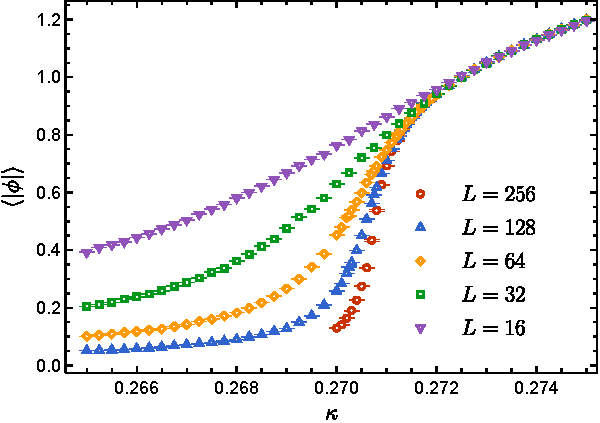
\includegraphics[width=0.5\textwidth]{orderparameter_2d_wolff_fahmc.pdf}
\caption{Order parameter $\langle|\bar\phi|\rangle$ as a function of the hopping parameter $\kappa$ for lattice sizes $L=16,\,32,\,64,\,128,\,256$ at $\lambda=0.022$. The transition becomes sharper with increasing volume.}
\label{fig:orderparameter_2d}
\end{figure}

The magnetic susceptibility $\chi$ is shown in \figs{fig:chi_2d_1}{fig:chi_2d_2}. The peak of $\chi$ grows with $L$ and shifts toward the critical $\kappa_c$, the expected finite-size scaling $\chi_{\max}\sim L^{\gamma/\nu}$ of the 2D Ising universality class ($\gamma/\nu = 7/4$).

\begin{figure}[t]
\centering
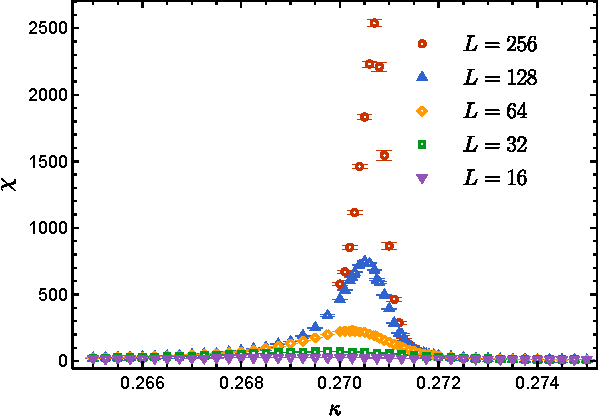
\includegraphics[width=0.5\textwidth]{chi_2d_wolff_fahmc_1.pdf}
\caption{Magnetic susceptibility $\chi$ as a function of $\kappa$ for different lattice sizes.}
\label{fig:chi_2d_1}
\end{figure}

\begin{figure}[t]
\centering
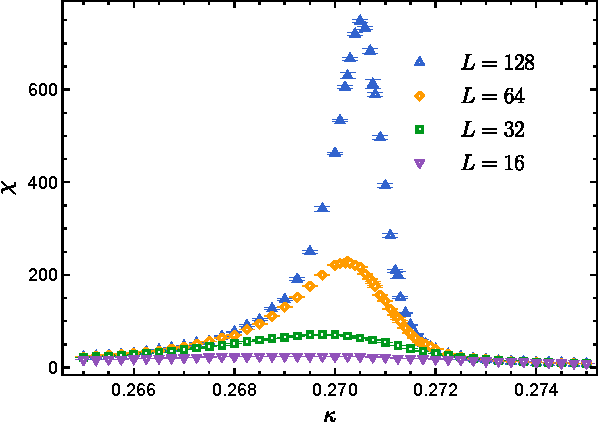
\includegraphics[width=0.5\textwidth]{chi_2d_wolff_fahmc_2.pdf}
\caption{Magnetic susceptibility $\chi$ (alternative representation) as a function of $\kappa$.}
\label{fig:chi_2d_2}
\end{figure}


The Binder cumulant $U_L$ is displayed in \fig{fig:binder_2d}. In the thermodynamic limit, $U_L\to 2/3$ in the broken phase and $U_L\to 0$ in the symmetric phase. Curves for different $L$ cross at the critical point $\kappa_c$, which is a powerful method for locating the phase transition independent of critical exponents.

\begin{figure}[t]
\centering
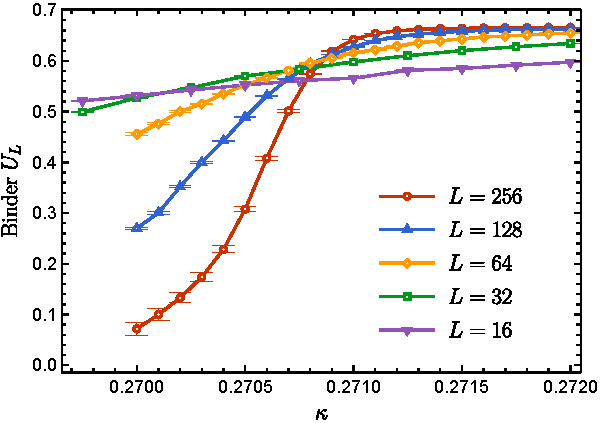
\includegraphics[width=0.5\textwidth]{binder_2d_wolff_fahmc.pdf}
\caption{Binder cumulant $U_L$ as a function of $\kappa$ for $L=16,\,32,\,64,\,128,\,256$. The crossing of curves at different $L$ determines the critical point $\kappa_c$.}
\label{fig:binder_2d}
\end{figure}


\fig{fig:bindercross_2d} shows the Binder crossing analysis. From the intersection of the $U_L$ curves for different lattice-size pairs, we extract the critical hopping parameter
\begin{equation}
\kappa_c(\lambda=0.022) \approx 0.27088,
\label{eq:kappa_c}
\end{equation}

\begin{figure}[t]
\centering
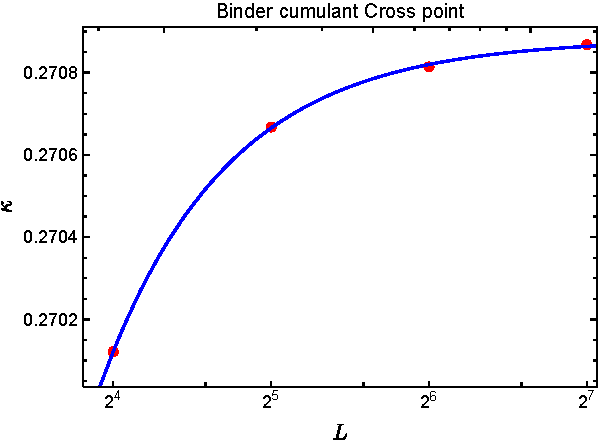
\includegraphics[width=0.5\textwidth]{bindercross_2d_wolff_fahmc.pdf}
\caption{Binder crossing analysis for the determination of $\kappa_c$. The intersection of different lattice-size pairs yields $\kappa_c\approx 0.27088$.}
\label{fig:bindercross_2d}
\end{figure}

\section{Critical point of 3D \texorpdfstring{$\phi^4$}{phi4} theory from Wolff + FA-HMC}
\label{sec:phi4_3d}

We extend the analysis to the three-dimensional $\phi^4$ theory on an $L^3$ cubic lattice. The lattice action takes the same form as \Eq{eq:phi4_action} with the sum over nearest neighbors running over $D=3$ directions. In three dimensions, we set the quartic coupling to $\lambda=0.9$. The $\mathbb{Z}_2$-breaking transition in 3D belongs to the 3D Ising universality class, with critical exponents $\nu\approx 0.63$.

\subsection{Simulation parameters}
\label{sec:3d_sim}


\subsection{Results}
\label{sec:3d_results}

\fig{fig:orderparameter_3d} shows the order parameter $\langle|\bar\phi|\rangle$ as a function of $\kappa$ for $L=8,\,16,\,32,\,64$. The crossover from the symmetric to the broken phase sharpens with increasing volume, analogous to the 2D case.

\begin{figure}[t]
\centering
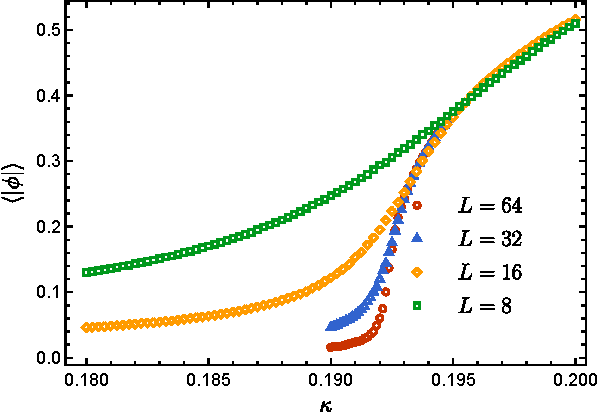
\includegraphics[width=0.5\textwidth]{orderparameter_3d_wolff_fahmc.pdf}
\caption{Order parameter $\langle|\bar\phi|\rangle$ vs.\ $\kappa$ for the 3D $\phi^4$ theory ($\lambda=0.9$) at lattice sizes $L=8,\,16,\,32,\,64$.}
\label{fig:orderparameter_3d}
\end{figure}

The magnetic susceptibility $\chi$ is displayed in \fig{fig:chi_3d}. The peak height grows with $L$ and its position converges toward $\kappa_c$.

\begin{figure}[t]
\centering
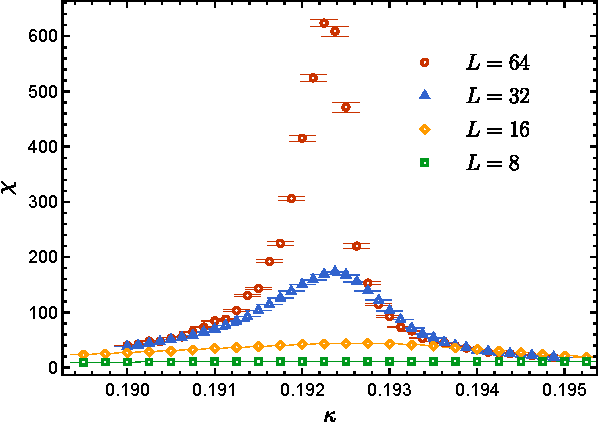
\includegraphics[width=0.5\textwidth]{chi_3d_wolff_fahmc.pdf}
\caption{Magnetic susceptibility $\chi$ vs.\ $\kappa$ for the 3D theory at different lattice sizes.}
\label{fig:chi_3d}
\end{figure}


The Binder cumulant $U_L$ is shown in \fig{fig:binder_3d}. Curves for different $L$ cross in a narrow region, pinpointing the critical hopping parameter. From the intersection of the $L=32$ and $L=64$ curves, we estimate
\begin{equation}
\kappa_c(\lambda=0.9) \approx 0.19225,
\label{eq:kappa_c_3d}
\end{equation}
consistent with $U_L^\ast\approx 2/3$ at the crossing, as expected for the 3D Ising universality class.

\begin{figure}[t]
\centering
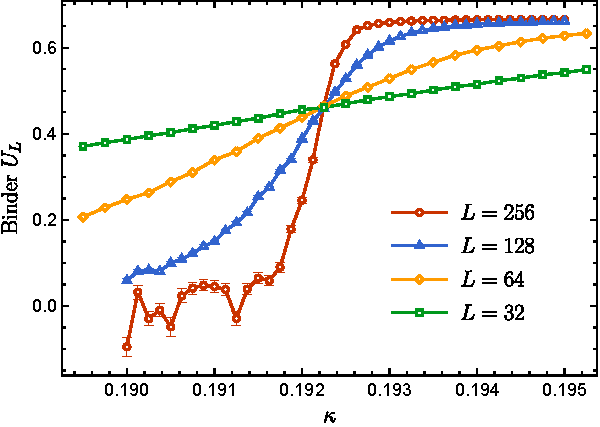
\includegraphics[width=0.5\textwidth]{binder_3d_wolff_fahmc.pdf}
\caption{Binder cumulant $U_L$ vs.\ $\kappa$ for the 3D $\phi^4$ theory at $L=8,\,16,\,32,\,64$. The crossing of curves for different $L$ determines $\kappa_c\approx 0.19225$.}
\label{fig:binder_3d}
\end{figure}


\section{Momentum-space propagator from diffusion models}
\label{sec:dm_propagator}

Having established the critical points for the 2D and 3D $\phi^4$ theories via Wolff + FA-HMC, we now test whether a score-based diffusion model can faithfully reproduce the momentum-space propagator $G(p)$.
We train a noise-conditional score network (NCSN++) on HMC-generated configurations at $L=128$ and $\lambda=0.022$, then generate independent samples by reverse-diffusion and compare the radially-averaged propagator
\begin{equation}
G(|p|) = \bigl\langle |\tilde\phi(p)|^2 \bigr\rangle_{\text{radial}}
\label{eq:propagator}
\end{equation}
against the HMC reference, where $\tilde\phi(p)$ is the discrete Fourier transform of a configuration. Errors are estimated via bootstrap.

We consider three representative values of the hopping parameter that span the phase diagram:
\begin{itemize}
\item $\kappa = 0.26$ --- in the symmetric phase;
\item $\kappa = 0.2705 \approx \kappa_c$ --- near the critical point;
\item $\kappa = 0.28$ --- in the broken phase.
\end{itemize}

%%% ---- NCSN++ Architecture Diagram ---- %%%
\begin{figure*}[t]
\centering

\includegraphics[width=\textwidth]{architecture_ncsnpp.pdf}
\caption{Architecture of the NCSN++ score network used for both 2D and 3D $\phi^4$ lattice field theory.
\textbf{(a)}~U-Net overview. The encoder (blue) consists of four ResBlock pairs at progressively coarser resolutions, separated by stride-2 convolutions (purple) that halve the spatial dimensions. The decoder (orange) mirrors this structure, upsampling via nearest-neighbor interpolation followed by a convolution (purple). Each encoder level provides two skip connections---from both sub-blocks---to the corresponding decoder level via channel concatenation (``concat~$\times 2$''). The diffusion time~$t$ is encoded by Gaussian Fourier projection (GFP) and a learned MLP, then injected additively into every ResBlock. The final output is divided by~$\sigma(t)$.
\textbf{(b)}~Internal structure of a single ResBlock; no residual connection is used. All convolutions use circular padding to enforce periodic boundary conditions.
For 2D fields all convolutions are \texttt{Conv2d}; for 3D they become \texttt{Conv3d} ($D=3$).}
\label{fig:architecture}
\end{figure*}

\subsection{Acceptance rate as a training diagnostic}
\label{sec:acceptance}

A natural quantitative measure of how well a diffusion model has learned the target distribution is the Metropolis--Hastings (MH) acceptance rate of a Metropolis-Adjusted Langevin Algorithm (MALA)~\cite{Roberts1998} that uses the score network as its proposal drift.

In the reverse-diffusion framework, the score network $s_\theta(\phi,t)\approx\nabla_\phi\log p_t(\phi)$ is trained to approximate the score of the noised distribution $p_t$. At small diffusion time $t\to 0$, $p_t\to p_0\propto e^{-S}$ and therefore $s_\theta(\phi,t)\to -\nabla_\phi S(\phi)$. From the current state $\phi_\tau$, the MALA proposal is
\begin{equation}
\psi_{\tau+1} = \phi_\tau + h\,s_\theta(\phi_\tau,\,t_{\text{mh}}) + \sqrt{2h}\,\eta,
\label{eq:mala_proposal}
\end{equation}
where $h$ is the step size, $t_{\text{mh}}$ the diffusion time at which the score is evaluated, and $\eta\sim\mathcal{N}(0,\mathds{1})$. Conditioned on $\phi_\tau$, the proposal is a Gaussian with mean $\phi_\tau + h\,s_\theta(\phi_\tau,t_{\text{mh}})$ and variance $2h\,I_n$, so the proposal kernel has the explicit form
\begin{widetext}
\begin{equation}
q(\psi_{\tau+1}|\phi_\tau) = \frac{1}{(4\pi h)^{n/2}}\exp\!\Bigl(-\frac{1}{4h}\bigl\|\psi_{\tau+1} - \phi_\tau - h\,s_\theta(\phi_\tau,t_{\text{mh}})\bigr\|^2\Bigr),
\label{eq:mala_kernel}
\end{equation}
\end{widetext}
where $n=L^D$ is the number of degrees of freedom and $p(\phi)\propto e^{-S(\phi)}$ is the known physical distribution. The accept-reject step is
\begin{equation}
\phi_{\tau+1} =
\begin{cases}
\psi_{\tau+1} & \text{with prob. } \min\!\bigl\{1,\,\tfrac{p(\psi_{\tau+1})\,q(\phi_\tau|\psi_{\tau+1})}{p(\phi_\tau)\,q(\psi_{\tau+1}|\phi_\tau)}\bigr\}, \\[6pt]
\phi_\tau      & \text{otherwise}.
\end{cases}
\label{eq:mala_accept}
\end{equation}
The transition probability ratio can be computed explicitly as
\begin{widetext}
\begin{equation}
\frac{p(\psi_{\tau+1})\,q(\phi_\tau|\psi_{\tau+1})}{p(\phi_\tau)\,q(\psi_{\tau+1}|\phi_\tau)}
= \exp\!\Bigl(
  -S(\psi_{\tau+1}) - \tfrac{1}{4h}\bigl\|\phi_\tau - \psi_{\tau+1} - h\,s_\theta(\psi_{\tau+1},t_{\text{mh}})\bigr\|^2
 + S(\phi_\tau) + \tfrac{1}{4h}\bigl\|\psi_{\tau+1} - \phi_\tau - h\,s_\theta(\phi_\tau,t_{\text{mh}})\bigr\|^2
\Bigr).
\label{eq:mala_ratio}
\end{equation}
\end{widetext}
Substituting the proposal \eq{eq:mala_proposal}, i.e.\ $\psi_{\tau+1}-\phi_\tau - h\,s_\theta(\phi_\tau) = \sqrt{2h}\,\eta$, the log acceptance probability simplifies to
\begin{widetext}
\begin{equation}
\log\alpha = \bigl[S(\phi_\tau)-S(\psi_{\tau+1})\bigr]
+ \tfrac{1}{2}\|\eta\|^2
- \tfrac{1}{4h}\bigl\|\sqrt{2h}\,\eta + h\bigl[s_\theta(\phi_\tau,t_{\text{mh}})+s_\theta(\psi_{\tau+1},t_{\text{mh}})\bigr]\bigr\|^2,
\label{eq:mala_logalpha}
\end{equation}
\end{widetext}
which is the form used in practice. The MH step guarantees that, regardless of the quality of $s_\theta$, the chain targets the correct distribution $e^{-S}$. The acceptance rate $\langle\min(1,e^{\log\alpha})\rangle$ therefore measures how closely the score-network proposal matches the true Langevin drift $-\nabla_\phi S$: a well-trained model yields a high acceptance rate, while a poorly trained one is rejected more often.

\paragraph{Parameter calibration.}
Two parameters must be chosen: the step size $h$ and the diffusion time $t_{\text{mh}}$. The calibration criterion is the \emph{diagnostic power}, defined as the difference in acceptance rate between a late-epoch (well-trained) and an early-epoch (poorly trained) checkpoint.

\paragraph{Step-size scaling.}
For MALA on a $d$-dimensional i.i.d.\ product target $\pi(x)=\prod_i f(x_i)$, Roberts and Rosenthal~\cite{Roberts1998} proved that the optimal proposal variance scales as $h\sim d^{-1/3}$, yielding an optimal acceptance rate of $0.574$. For a $D$-dimensional lattice with $d=L^D$ sites, this would give $h\sim L^{-D/3}$, i.e.\ $h\sim L^{-2/3}$ in 2D and $h\sim L^{-1}$ in 3D. However, the $\phi^4$ action contains nearest-neighbour couplings ($-2\kappa\sum_{\langle x,y\rangle}\phi_x\phi_y$) that strongly violate the i.i.d.\ assumption. The total action change for a global proposal scales as $\Delta S \sim d\cdot h$, so maintaining $\Delta S\sim O(1)$ for reasonable acceptance requires the RWM-type scaling $h\sim 1/d = 1/L^D$ rather than the MALA-optimal $d^{-1/3}$. Empirically, $h\sim L^{-D/3}$ produces a step size that is far too large in both 2D and 3D. We therefore adopt $h=c/L^D$ throughout, i.e.\ $h=c/L^2$ in 2D and $h=c/L^3$ in 3D, with the coefficient $c$ calibrated independently for each dimensionality.

We find that the diagnostic power is maximised at $t_{\text{mh}}=10^{-4}$, which is much smaller than values typically used in sampling ($t\sim 10^{-2}$). As shown in \fig{fig:calibrate_tmh}, at large $t_{\text{mh}}\gtrsim 5\times10^{-3}$ the gap reverses sign: the score at large $t$ approximates the score of a heavily smeared distribution $p_t\neq p_0$, so a well-trained model's proposal is rejected more often by the exact action than a poorly trained one whose drift is weak and effectively random. This reversal makes large $t_{\text{mh}}$ unsuitable as a diagnostic. For the step size in 2D, \fig{fig:calibrate_h} shows that $c=0.2$ (i.e.\ $h=0.2/L^2$) maximises the diagnostic power while keeping the late-epoch acceptance rate in the informative range $50$--$80\%$.

\begin{figure*}[t]
\centering
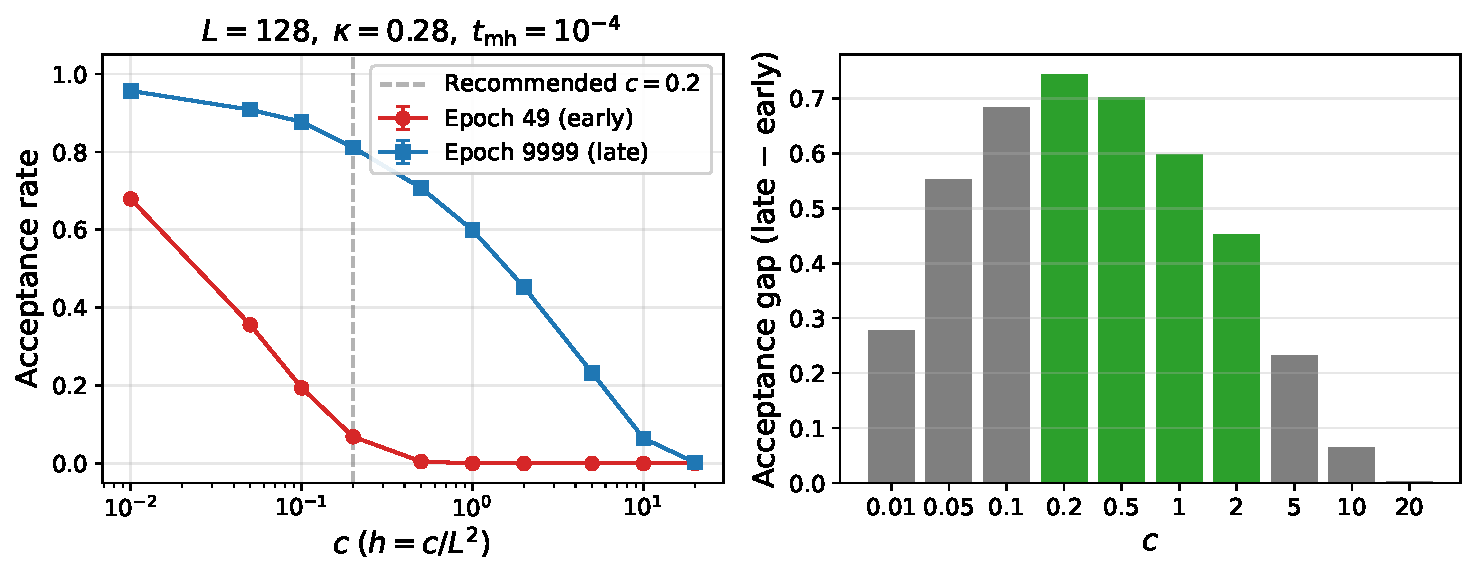
\includegraphics[width=\textwidth]{2Dphi4/calibrate_h_L128_k0.28.pdf}
\caption{Calibration of the MALA step size $h=c/L^2$ at $L=128$, $\kappa=0.28$, with $t_{\text{mh}}=10^{-4}$, $N=1024$ reference configurations and a single MH step. Left: acceptance rate vs.\ $c$ for the early-epoch (epoch~49, poorly trained) and late-epoch (epoch~9999, well-trained) checkpoints. Right: diagnostic power (acceptance gap between late and early checkpoints). Green bars indicate the ``useful'' range where the late-epoch acceptance rate is between $30\%$ and $85\%$.}
\label{fig:calibrate_h}
\end{figure*}

\begin{figure*}[t]
\centering
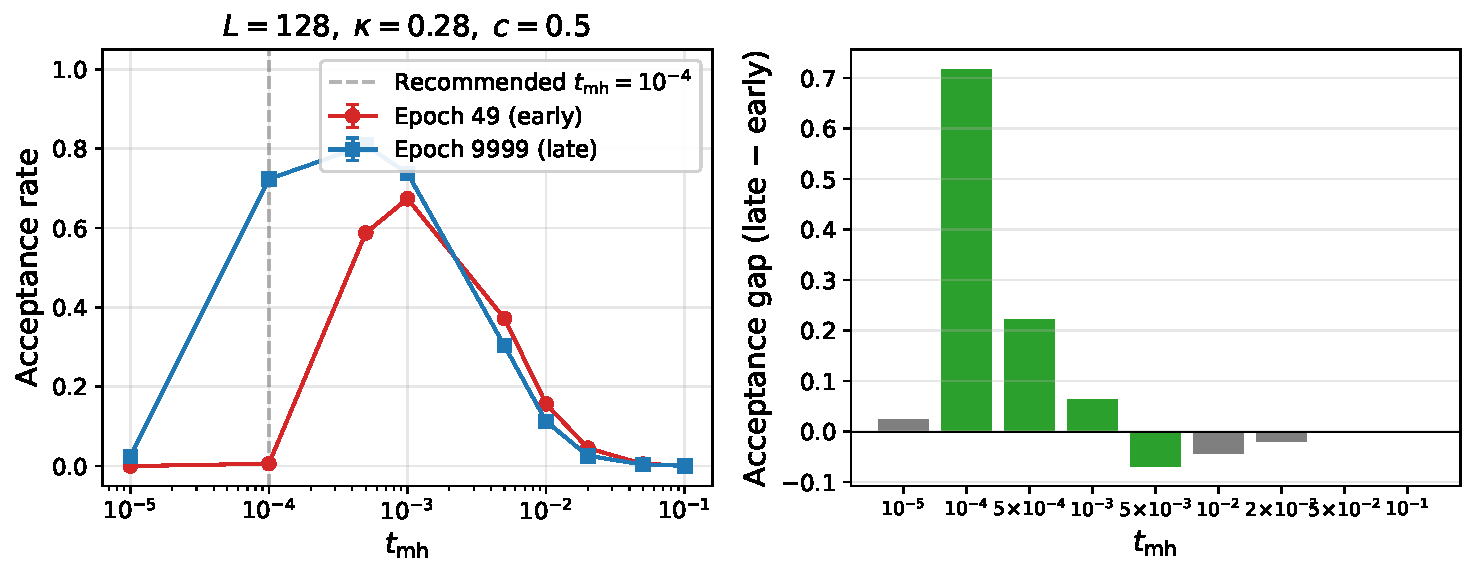
\includegraphics[width=0\textwidth]{2Dphi4/calibrate_t_mh_L128_k0.28.pdf}
\caption{Calibration of the evaluation time $t_{\text{mh}}$ at $L=128$, $\kappa=0.28$, with $c=0.2$, $N=1024$ and a single MH step. Left: acceptance rate vs.\ $t_{\text{mh}}$ for early (epoch~49) and late (epoch~9999) checkpoints. Right: diagnostic power. The gap reverses sign for $t_{\text{mh}}\gtrsim 5\times10^{-3}$, where the score network evaluates the gradient of a heavily smeared distribution rather than the physical action.}
\label{fig:calibrate_tmh}
\end{figure*}

With the calibrated parameters $c=0.2$ and $t_{\text{mh}}=10^{-4}$, we measure the MALA acceptance rate using $N=1024$ reference configurations drawn from the training data and a single MH step per configuration. Using a single MH step avoids the warm-up bias that arises with multiple steps (where the MH chain migrates toward lower-action regions, artificially inflating the acceptance rate) and maximises statistical independence across samples.

\paragraph{Acceptance rate during training.}
\fig{fig:acc_vs_epoch_2d} shows the acceptance rate as a function of training epoch for all three $\kappa$ values at $L=128$.
In all three cases, the acceptance rate starts near zero for the untrained model (epoch~49) and rises rapidly during the first $\sim$500 epochs, eventually fluctuating in the range $60$--$90\%$. The substantial epoch-to-epoch fluctuations reflect the stochastic nature of both the score-network training and the finite-sample MALA estimator, but the overall upward trend provides a clear signal that the score network progressively learns the correct Langevin drift.

\begin{figure}[t]
\centering
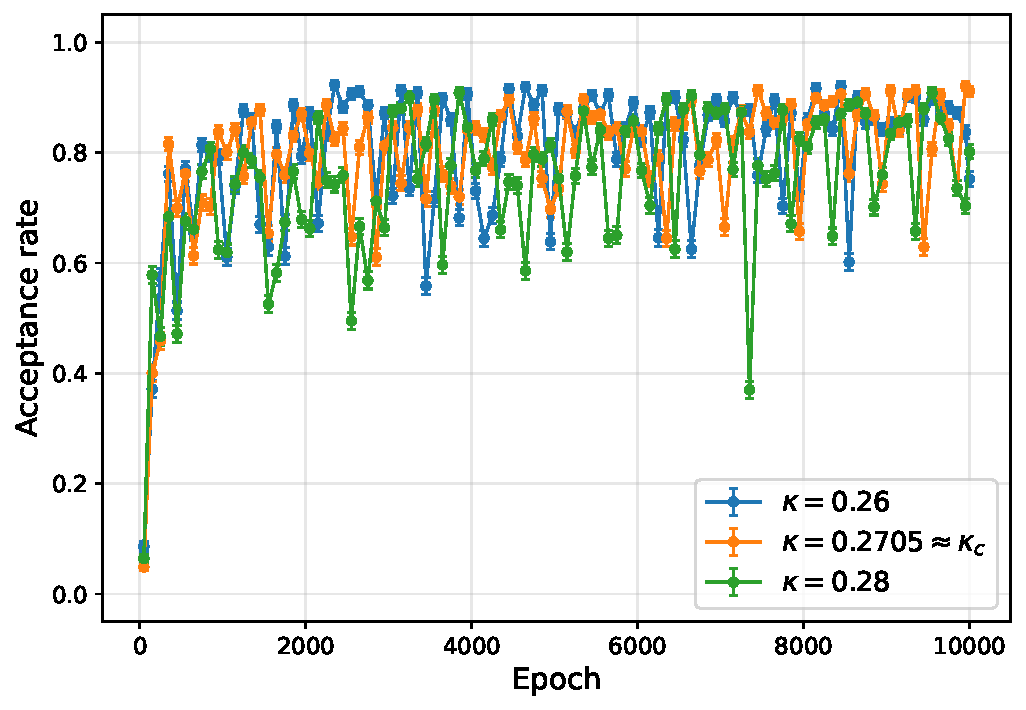
\includegraphics[width=0.5\textwidth]{2Dphi4/acceptance_vs_epoch_L128_combined.pdf}
\caption{MALA acceptance rate vs.\ training epoch for the 2D $\phi^4$ model at $L=128$, with $c=0.2$, $t_{\text{mh}}=10^{-4}$, $N=1024$ and a single MH step, for three values of $\kappa$ spanning the phase diagram.}
\label{fig:acc_vs_epoch_2d}
\end{figure}

\paragraph{Acceptance rate across lattice sizes.}
\Tabs{tab:acc_early}{tab:acc_late} summarise the average MALA acceptance rate for all trained models at two stages of training: an early window (epochs~49--249) and a late window (epochs~3999--4999). In all cases, the late-epoch acceptance rate is substantially higher than the early-epoch value, confirming that the diagnostic tracks training progress. The late-epoch acceptance rate increases mildly with lattice size, from $\sim 63$--$71\%$ at $L=8$ to $\sim 75$--$82\%$ at $L=64$--$128$. This trend is consistent with the $h=c/L^2$ scaling being slightly more conservative than the true optimal scaling for the correlated $\phi^4$ target: the optimal exponent likely lies between $L^{-2/3}$ (i.i.d.\ limit~\cite{Roberts1998}) and $L^{-2}$ (our choice), so at larger $L$ the step size is increasingly conservative and the acceptance rate rises accordingly. Despite this mild $L$-dependence, the acceptance rate remains a useful diagnostic at all lattice sizes tested.

\begin{table}[t]
\centering
\caption{Average MALA acceptance rate over epochs 49--249 (early training), with $c=0.2$, $t_{\text{mh}}=10^{-4}$, $N=1024$ and a single MH step.}
\label{tab:acc_early}
\begin{tabular}{cccc}
\toprule
$L$ & $\kappa=0.26$ & $\kappa=0.2705$ & $\kappa=0.28$ \\
\midrule
8   & $0.152$ & $0.136$ & $0.129$ \\
16  & $0.082$ & $0.228$ & $0.031$ \\
32  & $0.207$ & $0.205$ & $0.297$ \\
64  & $0.288$ & $0.375$ & $0.300$ \\
128 & $0.336$ & $0.325$ & $0.296$ \\
\bottomrule
\end{tabular}
\end{table}

\begin{table}[t]
\centering
\caption{Same as \Tab{tab:acc_early} but averaged over epochs 3999--4999 (late training).}
\label{tab:acc_late}
\begin{tabular}{cccc}
\toprule
$L$ & $\kappa=0.26$ & $\kappa=0.2705$ & $\kappa=0.28$ \\
\midrule
8   & $0.635$ & $0.715$ & $0.627$ \\
16  & $0.683$ & $0.641$ & $0.693$ \\
32  & $0.680$ & $0.753$ & $0.683$ \\
64  & $0.827$ & $0.818$ & $0.747$ \\
128 & $0.790$ & $0.792$ & $0.749$ \\
\bottomrule
\end{tabular}
\end{table}


\subsection{Direct score quality diagnostic}
\label{sec:score_quality}

While the MALA acceptance rate provides an effective indirect measure of score quality, it depends on the step size $h$ and evaluation time $t_{\text{mh}}$, requiring careful calibration (\fig{fig:calibrate_h}, \fig{fig:calibrate_tmh}).  A more direct diagnostic is to compare the model output $s_\theta(\phi,t)$ against the true gradient $-\nabla_\phi S(\phi)$ at a small diffusion time $t$, without any Metropolis--Hastings sampling.

For each reference configuration $\phi$ drawn from the training data, we evaluate the model score $s_\theta(\phi,t_{\text{eval}})$ at $t_{\text{eval}}=10^{-4}$ and compute the cosine similarity
\begin{equation}
C = \frac{\langle s_\theta,\, -\nabla S \rangle}{\|s_\theta\|\;\|\nabla S\|},
\label{eq:cos_sim}
\end{equation}
the relative mean-squared error $\|s_\theta - (-\nabla S)\|^2 / \|\nabla S\|^2$, and the magnitude ratio $\|s_\theta\|/\|\nabla S\|$, averaged over $N=512$ configurations. The choice $t_{\text{eval}}=10^{-4}$ (noise level $\sigma\approx 0.01$, or $0.5\%$ of the data range in normalised space) ensures that $p_t\approx p_0$ to high accuracy while the score estimate remains numerically stable. A larger evaluation time $t=0.01$ ($\sigma\approx 0.10$) introduces non-negligible Gaussian smoothing that systematically reduces the magnitude ratio below unity even for a perfectly trained model, making it a less informative diagnostic; a smaller time $t=10^{-5}$ ($\sigma\approx 0.003$) enters the regime where division by $\sigma(t)$ in the network output amplifies numerical noise.

\fig{fig:score_quality_2d} shows all three metrics as a function of training epoch for $L=128$ at all three $\kappa$ values. The cosine similarity rises from $\sim 0.99$ at epoch~49 to $\sim 0.998$ at late training; the relative MSE drops by more than an order of magnitude; and the magnitude ratio converges toward unity from above, starting at $\sim 1.5$ and reaching $\sim 0.9$--$1.0$ by epoch~5000. These trends are consistent with the monotonic improvement observed in the MALA acceptance rate (\fig{fig:acc_vs_epoch_2d}) and confirm that the score network progressively learns both the direction and the magnitude of $-\nabla S$.

\begin{figure*}[t]
\centering
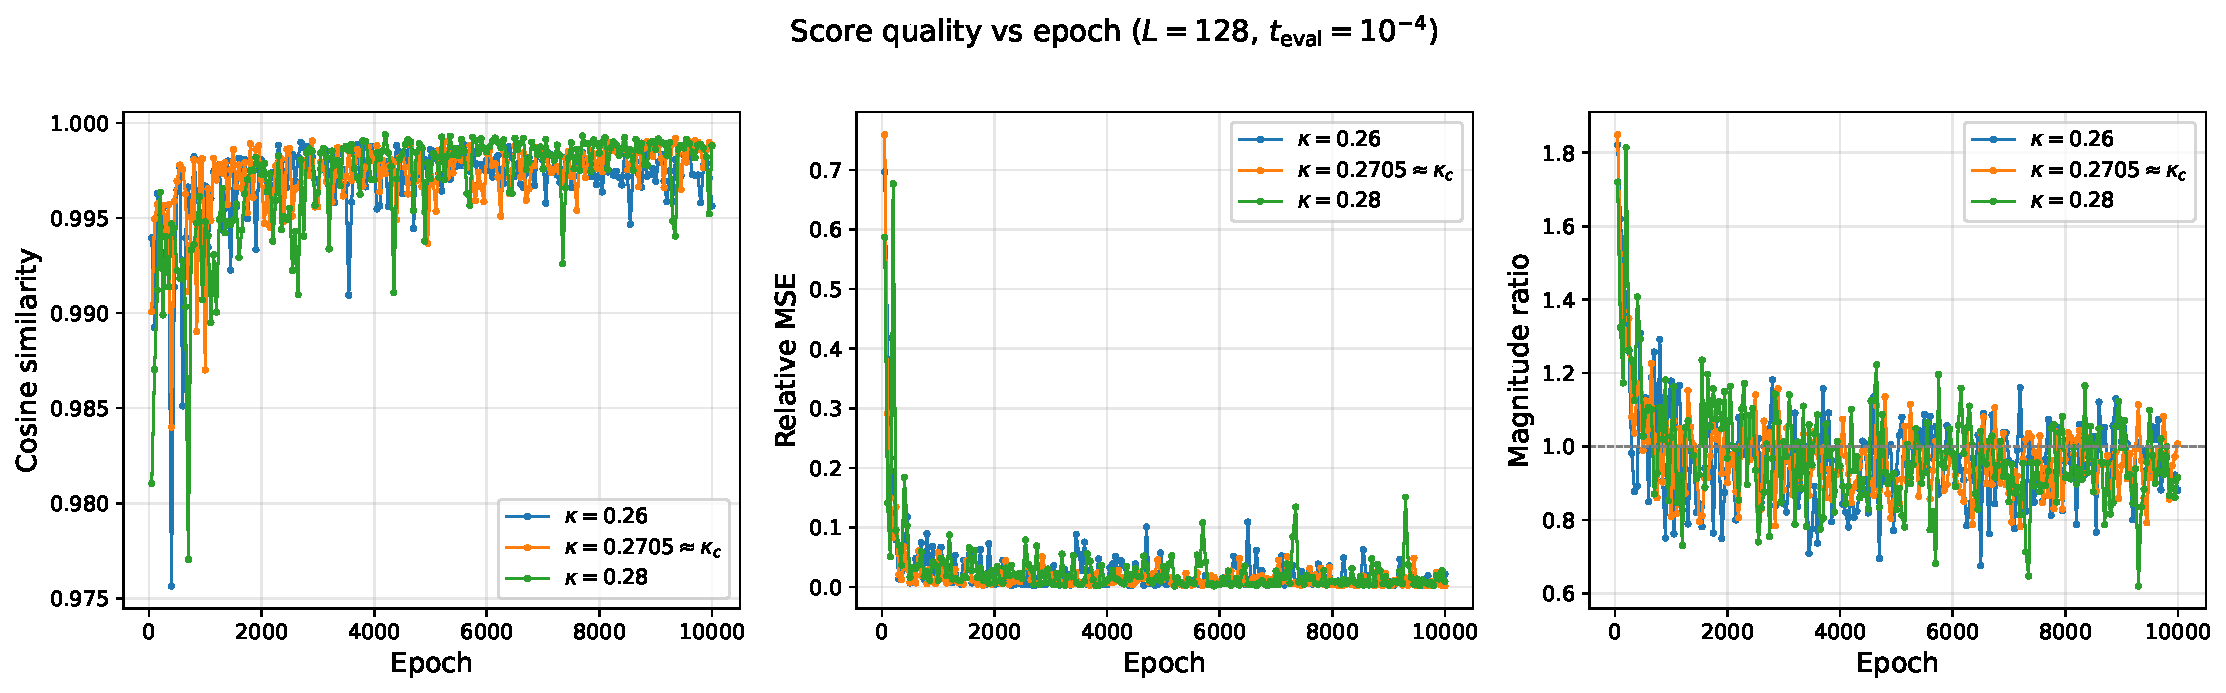
\includegraphics[width=\textwidth]{2Dphi4/score_quality_vs_epoch_L128_3panel.pdf}
\caption{Score quality vs.\ training epoch for the 2D $\phi^4$ model at $L=128$, evaluated at $t=10^{-4}$ with $N=512$ reference configurations. Left: cosine similarity. Centre: relative MSE. Right: magnitude ratio (dashed line indicates the ideal value of $1$).}
\label{fig:score_quality_2d}
\end{figure*}

\Tabs{tab:score_early}{tab:score_late} summarise the average cosine similarity and magnitude ratio across all lattice sizes and $\kappa$ values, in the same early and late training windows used for the acceptance rate (\Tabs{tab:acc_early}{tab:acc_late}). In the early window (epochs~49--249), the magnitude ratio is $\sim 1.4$--$2.1$, indicating that the untrained model significantly overshoots the true gradient magnitude. By late training (epochs~3999--4999), the magnitude ratio converges to $0.9$--$1.1$ for $L\ge 32$, confirming quantitative accuracy of the learned score. For $L=8$ and $16$ a slight residual overshoot ($\sim 1.1$--$1.3$) persists, likely reflecting the smaller number of degrees of freedom where the model has less room to average out local fluctuations.

\begin{table}[t]
\centering
\caption{Average cosine similarity $C$ and magnitude ratio $\|s_\theta\|/\|\nabla S\|$ over epochs 49--249 (early training), evaluated at $t=10^{-4}$ with $N=512$ reference configurations.}
\label{tab:score_early}
\begin{tabular}{ccccccc}
\toprule
 & \multicolumn{3}{c}{Cosine similarity $C$} & \multicolumn{3}{c}{Magnitude ratio} \\
\cmidrule(lr){2-4} \cmidrule(lr){5-7}
$L$ & $\kappa\!=\!0.26$ & $0.2705$ & $0.28$ & $\kappa\!=\!0.26$ & $0.2705$ & $0.28$ \\
\midrule
8   & $0.987$ & $0.971$ & $0.974$ & $2.102$ & $2.018$ & $1.942$ \\
16  & $0.985$ & $0.977$ & $0.976$ & $2.046$ & $1.716$ & $2.042$ \\
32  & $0.981$ & $0.981$ & $0.986$ & $1.704$ & $1.647$ & $1.568$ \\
64  & $0.992$ & $0.985$ & $0.990$ & $1.581$ & $1.401$ & $1.408$ \\
128 & $0.994$ & $0.994$ & $0.989$ & $1.512$ & $1.472$ & $1.459$ \\
\bottomrule
\end{tabular}
\end{table}

\begin{table}[t]
\centering
\caption{Same as \Tab{tab:score_early} but averaged over epochs 3999--4999 (late training).}
\label{tab:score_late}
\begin{tabular}{ccccccc}
\toprule
 & \multicolumn{3}{c}{Cosine similarity $C$} & \multicolumn{3}{c}{Magnitude ratio} \\
\cmidrule(lr){2-4} \cmidrule(lr){5-7}
$L$ & $\kappa\!=\!0.26$ & $0.2705$ & $0.28$ & $\kappa\!=\!0.26$ & $0.2705$ & $0.28$ \\
\midrule
8   & $0.988$ & $0.991$ & $0.990$ & $1.282$ & $1.148$ & $1.267$ \\
16  & $0.989$ & $0.989$ & $0.993$ & $1.119$ & $1.158$ & $1.052$ \\
32  & $0.988$ & $0.993$ & $0.990$ & $1.053$ & $1.014$ & $0.953$ \\
64  & $0.996$ & $0.996$ & $0.996$ & $0.968$ & $0.972$ & $0.949$ \\
128 & $0.997$ & $0.997$ & $0.998$ & $0.907$ & $0.938$ & $0.950$ \\
\bottomrule
\end{tabular}
\end{table}


\subsection{Training loss for 3D \texorpdfstring{$\phi^4$}{phi4}}
\label{sec:dm_training}

We train the NCSN++ model on Wolff + FA-HMC configurations of the 3D theory at $L=64$ and $\lambda=0.9$ for three hopping parameters: $\kappa=0.18$ (symmetric phase), $\kappa=0.1923\approx\kappa_c$ (near the critical point), and $\kappa=0.2$ (broken phase). The score-matching loss is decomposed by the diffusion time $t$ into a UV component ($t<0.2$, probing short-distance modes), an intermediate component ($0.2<t<0.8$), and an IR component ($t>0.8$, probing long-distance modes).

\fig{fig:loss_3d_L64} shows the training loss evolution up to 20000 epochs. The total loss (panel a) converges for all three $\kappa$ values, with a clear hierarchy: the symmetric-phase model ($\kappa=0.18$) has the highest loss plateau, while the broken-phase model ($\kappa=0.2$) converges to the lowest value. The decomposition reveals that the IR loss (panel d) is the dominant contribution and the most sensitive to $\kappa$: the symmetric phase shows the largest IR loss, reflecting the challenge of learning long-wavelength modes when the correlation length is large but finite. The mid and UV components (panels b, c) show a similar ordering, confirming that the phase-dependent difficulty extends across all noise levels.

\begin{figure*}[t]
\centering
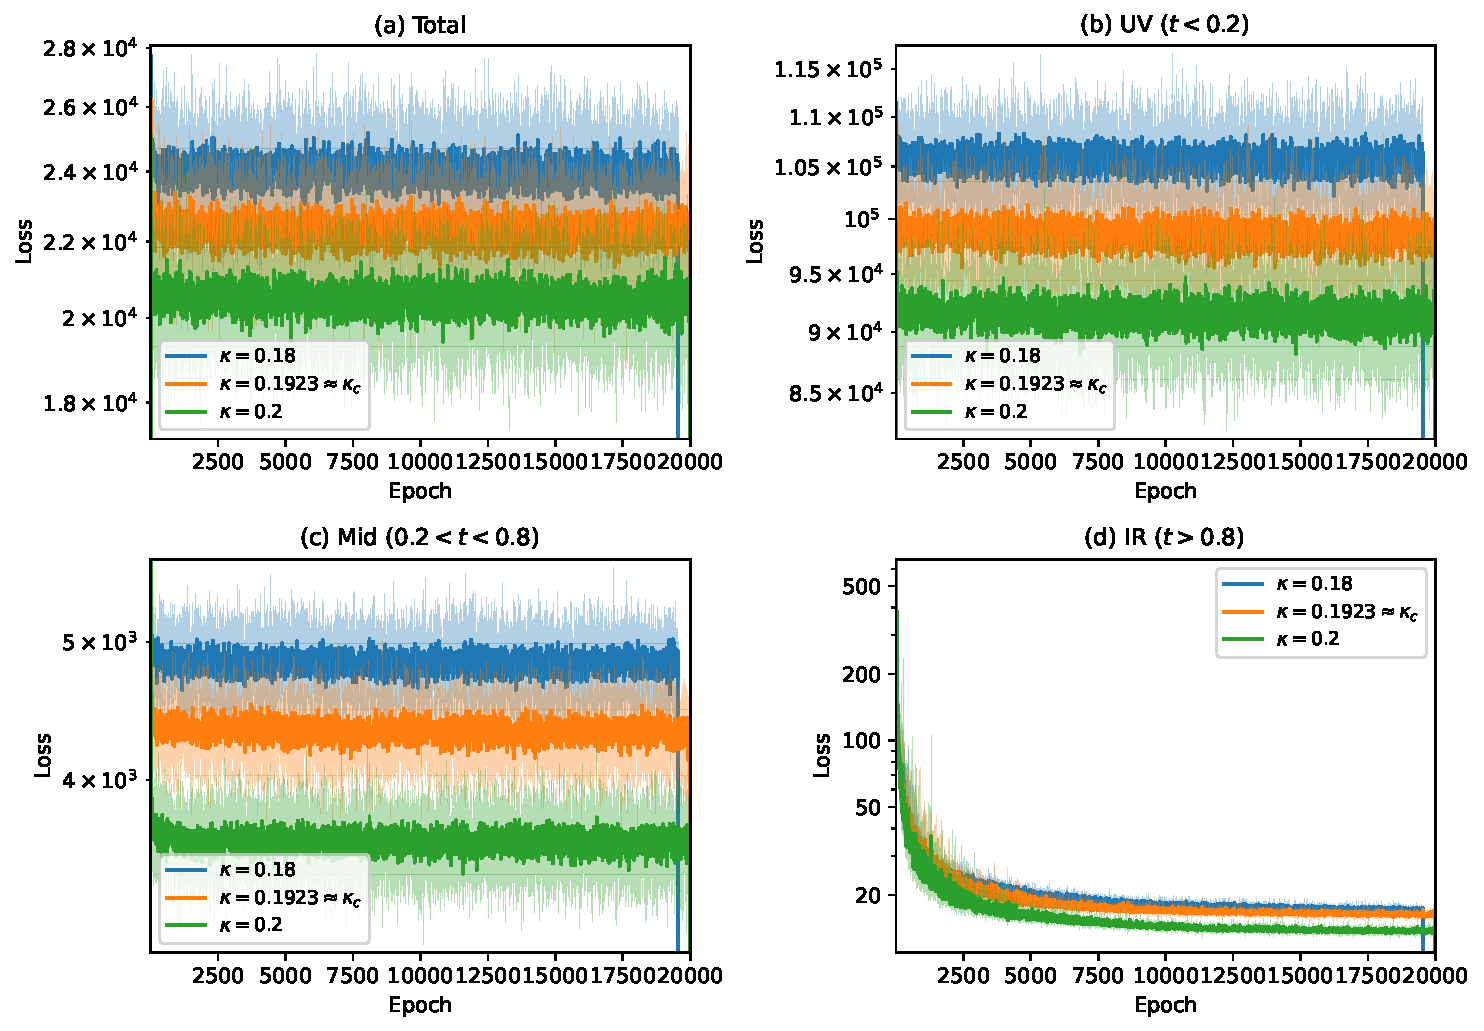
\includegraphics[width=\textwidth]{3Dphi4/loss_3d_L64_decomposed.pdf}
\caption{Training loss vs.\ epoch for the 3D $\phi^4$ NCSN++ diffusion model at $L=64$, $\lambda=0.9$: (a) total loss, (b) UV component ($t<0.2$), (c) mid component ($0.2<t<0.8$), (d) IR component ($t>0.8$). Each panel compares three $\kappa$ values spanning the phase diagram.}
\label{fig:loss_3d_L64}
\end{figure*}


\subsection{Acceptance rate for 3D \texorpdfstring{$\phi^4$}{phi4}}
\label{sec:acc_3d}

We apply the same MALA acceptance-rate diagnostic to the 3D models at $L=64$, $\lambda=0.9$, now with $h=c/L^3$ and $N=256$ reference configurations. \fig{fig:calibrate_h_3d} shows the step-size calibration: the optimal coefficient is again $c=0.2$, the same value found in 2D. This consistency strongly supports the $h=c/L^D$ scaling: the coefficient $c$ is universal across spatial dimensions once the volume factor $L^D$ is correctly accounted for. The $t_{\text{mh}}$ calibration (\fig{fig:calibrate_tmh_3d}) with $c=0.5$ confirms that $t_{\text{mh}}=10^{-4}$ maximises the diagnostic power, as in the 2D case.

\begin{figure*}[t]
\centering
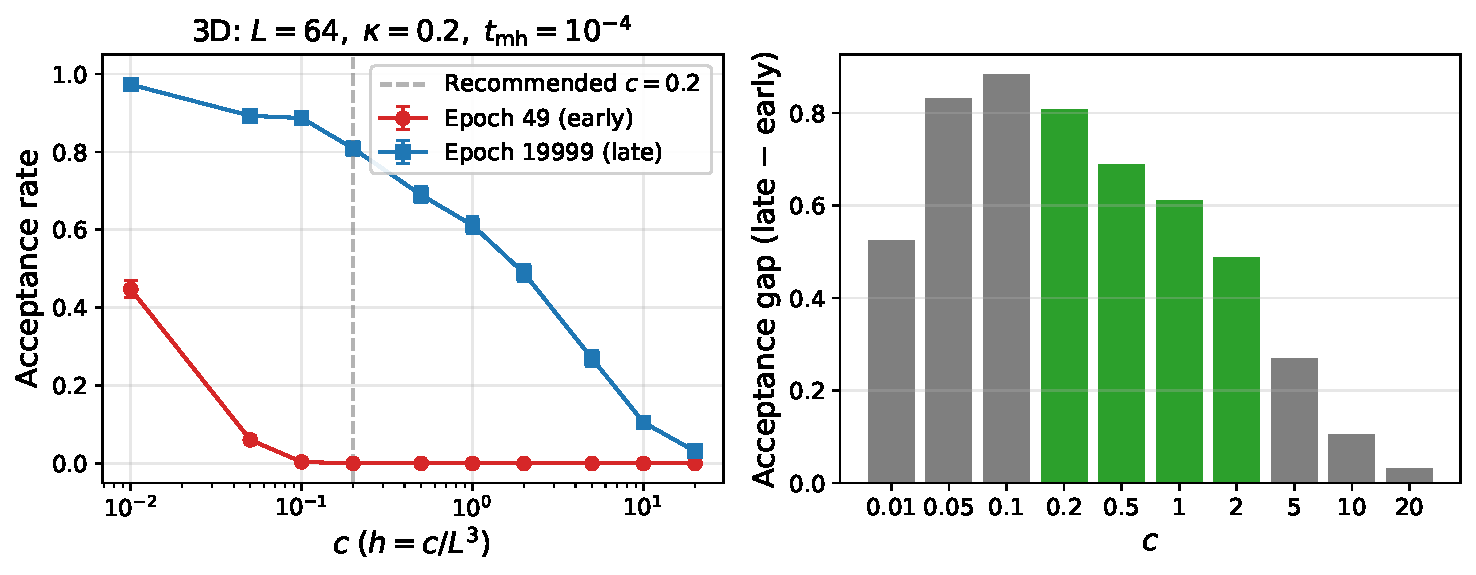
\includegraphics[width=\textwidth]{3Dphi4/calibrate_h_3d_L64_k0.2.pdf}
\caption{Calibration of the MALA step size $h=c/L^3$ for the 3D $\phi^4$ model at $L=64$, $\kappa=0.2$, $\lambda=0.9$, with $t_{\text{mh}}=10^{-4}$, $N=256$ and a single MH step. The optimal $c=0.2$ matches the 2D result, validating the $h=c/L^D$ scaling.}
\label{fig:calibrate_h_3d}
\end{figure*}

\begin{figure*}[t]
\centering
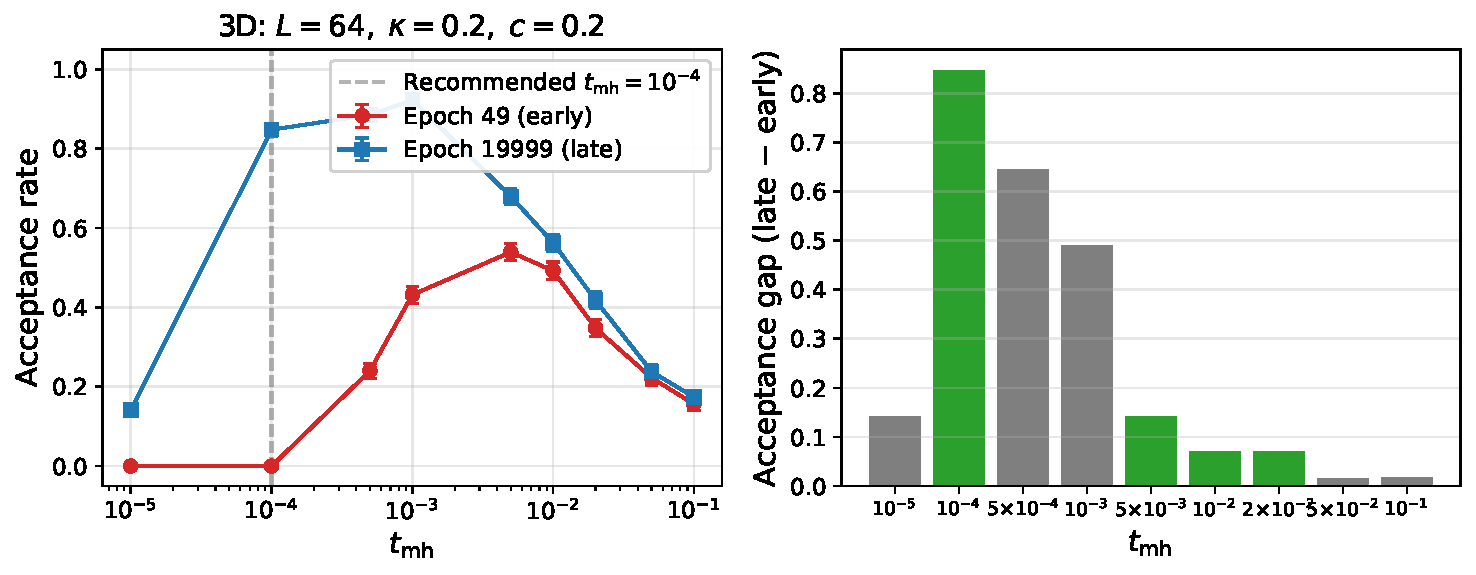
\includegraphics[width=\textwidth]{3Dphi4/calibrate_t_mh_3d_L64_k0.2.pdf}
\caption{Calibration of $t_{\text{mh}}$ for the 3D model at $L=64$, $\kappa=0.2$, with $c=0.5$ and $h=c/L^3$, $N=256$ and a single MH step.}
\label{fig:calibrate_tmh_3d}
\end{figure*}

\fig{fig:acc_vs_epoch_3d} shows the acceptance rate vs.\ training epoch for all three 3D models with $c=0.5$. The acceptance rates reach $60$--$90\%$ at late epochs, comparable to the 2D results and confirming that the $h=c/L^D$ scaling yields a consistent diagnostic across dimensions.

\begin{figure}[t]
\centering
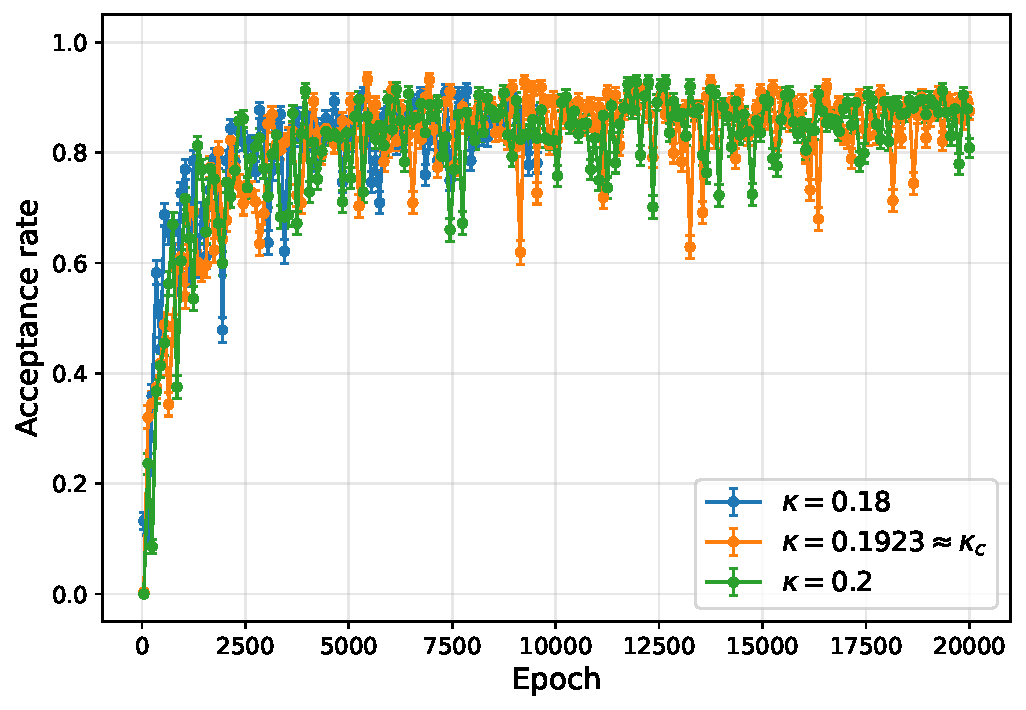
\includegraphics[width=0.5\textwidth]{3Dphi4/acceptance_vs_epoch_3d_L64_combined.pdf}
\caption{MALA acceptance rate vs.\ training epoch for the 3D $\phi^4$ model at $L=64$, $\lambda=0.9$, with $c=0.5$, $h=c/L^3$, $t_{\text{mh}}=10^{-4}$, $N=256$ and a single MH step.}
\label{fig:acc_vs_epoch_3d}
\end{figure}

\paragraph{Direct score quality for 3D.}
We apply the same direct score-quality diagnostic to the 3D models, evaluating the cosine similarity, relative MSE, and magnitude ratio at $t_{\text{eval}}=10^{-4}$ with $N=64$ reference configurations. \fig{fig:score_quality_3d} shows the three metrics as a function of training epoch for all three $\kappa$ values. The cosine similarity rises from $\sim 0.96$ at early training to $\sim 0.995$ at late training; the relative MSE drops by more than an order of magnitude; and the magnitude ratio converges to $\sim 0.97$--$1.00$ from an initial overshoot of $\sim 1.4$--$1.5$. These trends mirror the 2D results (\fig{fig:score_quality_2d}) and confirm that the score network learns both the direction and the magnitude of $-\nabla S$ in three dimensions.

\begin{figure*}[t]
\centering
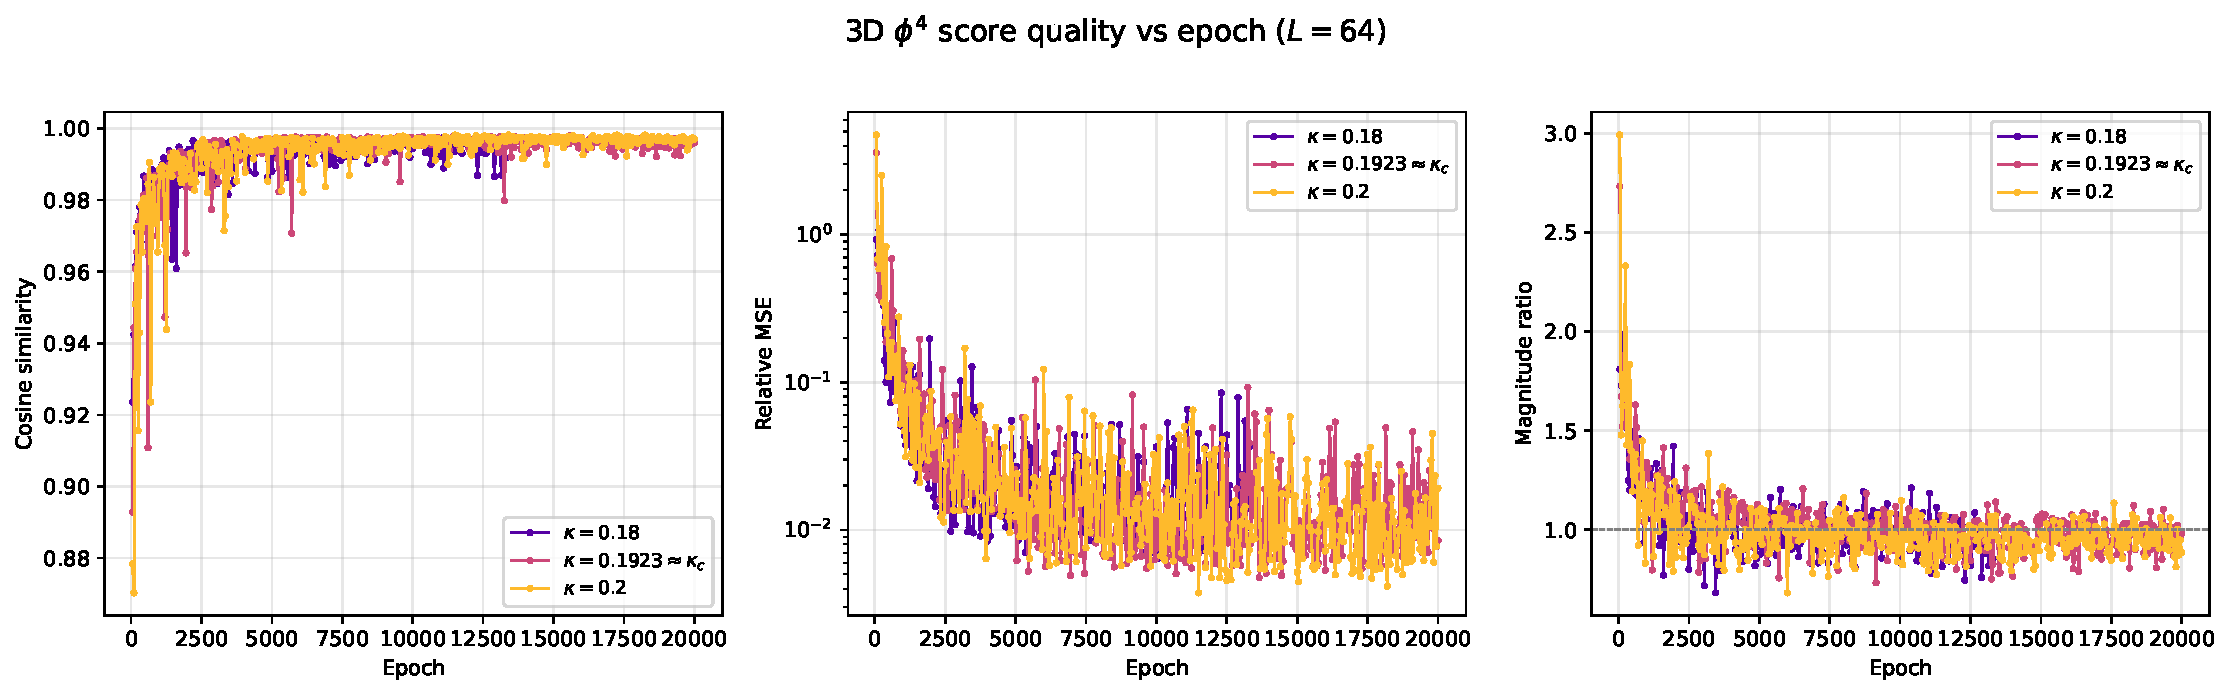
\includegraphics[width=\textwidth]{3Dphi4/score_quality_3d_3panel.pdf}
\caption{Score quality vs.\ training epoch for the 3D $\phi^4$ model at $L=64$, $\lambda=0.9$, evaluated at $t=10^{-4}$ with $N=64$ reference configurations. Left: cosine similarity. Centre: relative MSE. Right: magnitude ratio.}
\label{fig:score_quality_3d}
\end{figure*}


\subsection{\texorpdfstring{$\kappa=0.26$}{kappa=0.26}: symmetric phase}
\label{sec:prop_026}

\fig{fig:prop_026_log} shows the propagator for $\kappa=0.26$ at several training epochs compared to the HMC baseline. The diffusion model converges to the HMC propagator as training progresses, with the largest deviations observed at early epochs and at small momenta (large correlation lengths).

\begin{figure*}[t]
\centering
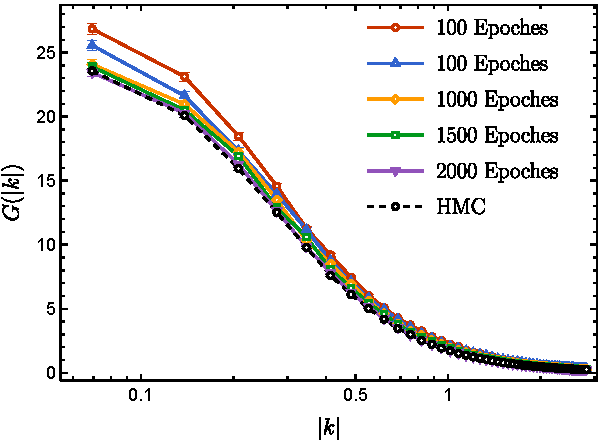
\includegraphics[width=0.5\textwidth]{2Dphi4/correlation_k=0.26/prop_k=0.26_log.pdf}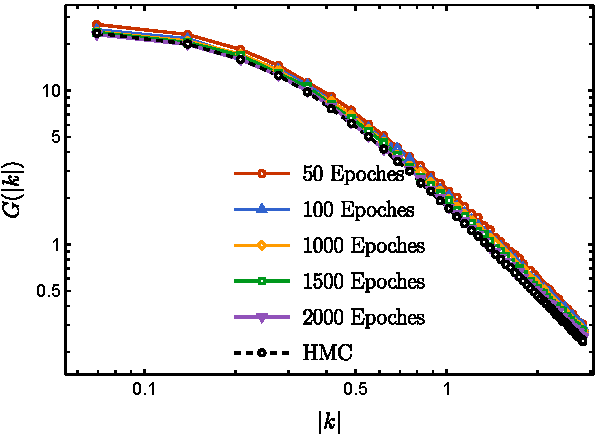
\includegraphics[width=0.5\textwidth]{2Dphi4/correlation_k=0.26/prop_k=0.26_log_log.pdf}
\caption{Momentum-space propagator $G(p)$ for $\kappa=0.26$ (symmetric phase), $L=128$. Semi-log (left) and double-logarithmic (right) comparison of HMC and DM at different training epochs.}
\label{fig:prop_026_log}
\end{figure*}



\subsection{\texorpdfstring{$\kappa=0.2705$}{kappa=0.2705}: near-critical regime}
\label{sec:prop_02705}

Near the critical point $\kappa\approx\kappa_c$, the correlation length diverges and the propagator develops a power-law tail $G(p)\sim p^{-(2-\eta)}$ at small momenta, making it the most demanding test case.
\fig{fig:prop_02705_log} demonstrates that the diffusion model successfully captures this behavior, with the DM propagator approaching the HMC result upon sufficient training.

\begin{figure*}[t]
\centering
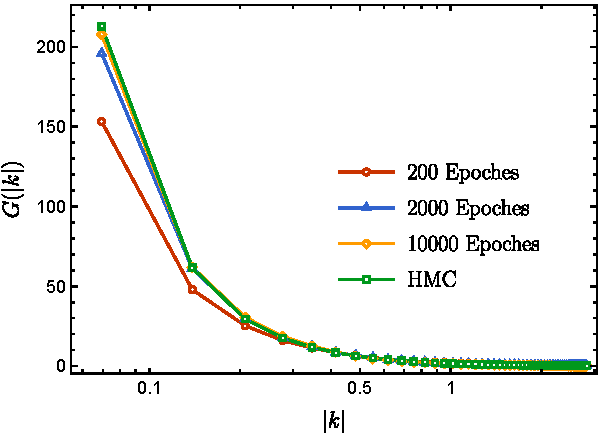
\includegraphics[width=0.5\textwidth]{2Dphi4/correlation_k=0.2705/prop_k=0.2705_log.pdf}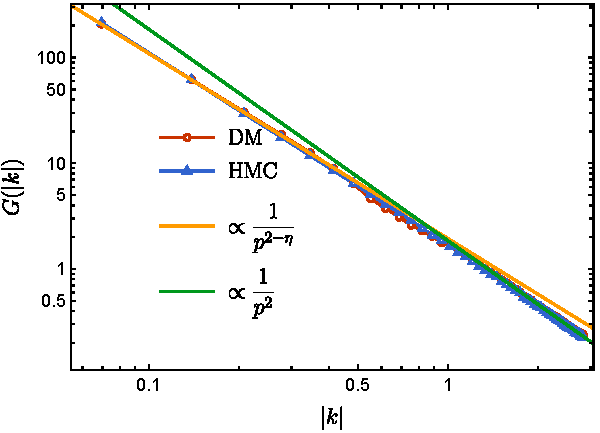
\includegraphics[width=0.5\textwidth]{2Dphi4/correlation_k=0.2705/prop_k=0.2705_log_log.pdf}
\caption{Propagator $G(p)$ at $\kappa=0.2705\approx\kappa_c$ (near-critical), $L=128$. Semi-log (left) and double-logarithmic (right) comparison of HMC and DM at different training epochs.}
\label{fig:prop_02705_log}
\end{figure*}


\subsection{\texorpdfstring{$\kappa=0.28$}{kappa=0.28}: broken phase}
\label{sec:prop_028}

In the ordered phase at $\kappa=0.28$, the propagator acquires a large zero-mode contribution and a mass gap. \fig{fig:prop_028_log} shows that the diffusion model also reproduces the propagator faithfully in this regime.

\begin{figure*}[t]
\centering
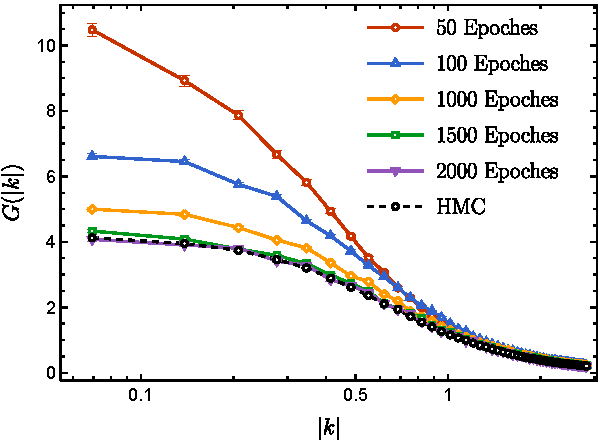
\includegraphics[width=0.5\textwidth]{2Dphi4/correlation_k=0.28/prop_k=0.28_log.pdf}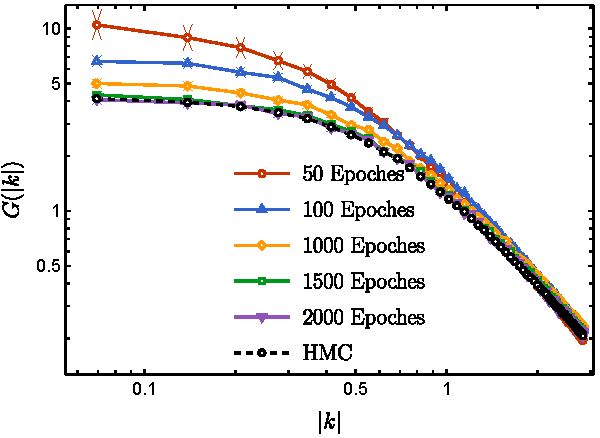
\includegraphics[width=0.5\textwidth]{2Dphi4/correlation_k=0.28/prop_k=0.28_log_log.pdf}
\caption{Propagator $G(p)$ for $\kappa=0.28$ (broken phase), $L=128$. Semi-log (left) and double-logarithmic (right) comparison of HMC and DM at different training epochs.}
\label{fig:prop_028_log}
\end{figure*}



\bibliography{ref-lib}

\end{document}
%
% ****** End of file apssamp.tex ******
